\label{ap:ap02}
\chapter{Linguagem de Programação Aplicada}

\section*{\textbf{A - ENUNCIADO}}
\textbf{Nome da base de dados do exercício}: \textit{precos\_carros\_brasil.csv}

\textbf{Informações sobre a base de dados: }

Dados dos preços médios dos carros brasileiros, das mais diversas marcas, no ano de 2021, de acordo com dados extraídos
da tabela FIPE (Fundação Instituto de Pesquisas Econômicas). A base original foi extraída do site Kaggle
(\href{https://www.kaggle.com/datasets/vagnerbessa/average-car-prices-bazil/data}{\textcolor[HTML]{1155CC}{Acesse aqui
a base original}}). A mesma foi adaptada para ser utilizada no presente exercício.

Observação: As variáveis \textit{fuel\hspace{0pt}\hspace{0pt}}, \textit{gear} e \textit{engine\_size} foram extraídas
dos valores da coluna \textit{model}, pois na base de dados original não há coluna dedicada a esses valores. Como
alguns valores do modelo não contêm as informações do tamanho do motor, este conjunto de dados não contém todos os
dados originais da tabela FIPE.

\textbf{Metadados:}
\begin{center}
\begin{tabular}{|p{0.4\textwidth}|p{0.55\textwidth}|}
\hline
\textbf{Nome do campo} & \textbf{Descrição} \\
\hline
year\_of\_reference & O preço médio corresponde a um mês do ano de referência \\
\hline
month\_of\_reference & O preço médio corresponde a um mês específico, pois a FIPE atualiza mensalmente \\
\hline
fipe\_code & Código único da FIPE \\
\hline
authentication & Código único de autenticação para consulta FIPE \\
\hline
brand & Marca do carro \\
\hline
model & Modelo do carro \\
\hline
fuel & Tipo de combustível \\
\hline
gear & Tipo de engrenagem \\
\hline
engine\_size & Tamanho do motor em centímetros cúbicos \\
\hline
year\_model & Ano do modelo (pode ser diferente do ano de fabricação) \\
\hline
avg\_price & Preço médio do carro em reais \\
\hline
\end{tabular}
\end{center}



\textbf{\textit{Atenção: ao fazer o download da base de dados, selecione o formato .csv. É o formato que será
considerado correto na resolução do exercício.}}



\newpage
\subsection*{\textbf{1 Análise Exploratória dos dados}}
%\textbf{1 Análise Exploratória dos dados}



A partir da base de dados \textbf{precos\_carros\_brasil.csv}, execute as seguintes tarefas:

\begin{enumerate}[series=listWWNumxi,label=\alph*.,ref=\alph*]
\item Carregue a base de dados media\_precos\_carros\_brasil.csv
\item Verifique se há valores faltantes nos dados. Caso haja, escolha uma tratativa para resolver o problema de valores
faltantes
\item Verifique se há dados duplicados nos dados
\item Crie duas categorias, para separar colunas numéricas e categóricas. Imprima o resumo de informações das variáveis
numéricas e categóricas (estatística descritiva dos dados)
\item Imprima a contagem de valores por modelo (model) e marca do carro (brand)
\item Dê um breve explicação (máximo de quatro linhas) sobre os principais resultados encontrados na Análise
Exploratória dos dados
\end{enumerate}


\subsection*{\textbf{2 Visualização dos dados}}
%\textbf{2 Visualização dos dados}

A partir da base de dados \textbf{precos\_carros\_brasil.csv,} execute as seguintes tarefas:

\begin{enumerate}[series=listWWNumx,label=\alph*.,ref=\alph*]
\item Gere um gráfico da distribuição da quantidade de carros por marca
\item Gere um gráfico da distribuição da quantidade de carros por tipo de engrenagem do carro
\item Gere um gráfico da evolução da média de preço dos carros ao longo dos meses de 2022 (variável de tempo no eixo X)
\item Gere um gráfico da distribuição da média de preço dos carros por marca e tipo de engrenagem
\item Dê uma breve explicação (máximo de quatro linhas) sobre os resultados gerados no item d
\item Gere um gráfico da distribuição da média de preço dos carros por marca e tipo de combustível
\item Dê uma breve explicação (máximo de quatro linhas) sobre os resultados gerados no item f
\end{enumerate}






\subsection*{\textbf{3 Aplicação de modelos de machine learning para prever o preço médio dos carros}}
%\textbf{3 Aplicação de modelos de machine learning para prever o preço médio dos carros}




{\centering
A partir da base de dados \textbf{precos\_carros\_brasil.csv}, execute as seguintes tarefas:
\par}

\begin{enumerate}[series=listWWNumxii,label=\alph*.,ref=\alph*]
\item Escolha as variáveis \textbf{numéricas} (modelos de Regressão) para serem as variáveis independentes do modelo.A
variável target é \textbf{avg\_price. Observação:} caso julgue necessário, faça a transformação de variáveis
categóricas em variáveis numéricas para inputar no modelo. Indique \textbf{quais variáveis} foram transformadas e
\textbf{como} foram transformadas
\item Crie partições contendo 75\% dos dados para treino e 25\% para teste
\item Treine modelos RandomForest (biblioteca RandomForestRegressor) e XGBoost (biblioteca XGBRegressor) para predição
dos preços dos carros. \textbf{Observação}: caso julgue necessário, mude os parâmetros dos modelos e rode novos
modelos. Indique quais parâmetros foram inputados e indique o treinamento de cada modelo
\item Grave os valores preditos em variáveis criadas
\item Realize a análise de importância das variáveis para estimar a variável target, \textbf{para cada modelo treinado}
\item Dê uma breve explicação (máximo de quatro linhas) sobre os resultados encontrados na análise de importância de
variáveis
\item Escolha o melhor modelo com base nas métricas de avaliação MSE, MAE e R²
\item Dê uma breve explicação (máximo de quatro linhas) sobre qual modelo gerou o melhor resultado e a métrica de
avaliação utilizada
\end{enumerate}

\section*{\textbf{B - RESOLUÇÃO}}

\subsection*{\textbf{1 Análise Exploratória dos dados}}
\begin{adjustwidth}{1em}{}
\textbf{a. Carregue a base de dados media\_precos\_carros\_brasil.csv}
\end{adjustwidth}

\lstset{
  basicstyle=\ttfamily\small,
  keywordstyle=\color{blue},
  commentstyle=\color{gray},
  stringstyle=\color{red},
  showstringspaces=false,
  breaklines=true,
  frame=single,
  language=Python
}
\lstdefinestyle{output}{
  basicstyle=\small\ttfamily,
  numbers=none,
  frame=tblr,
  columns=fullflexible,
  backgroundcolor=\color{blue!10},             
  keepspaces=true,   
  linewidth=0.9\linewidth,
  xleftmargin=0.1\linewidth,
  %basicstyle=\ttfamily\scriptsize,
  breaklines=true
}
\lstdefinestyle{input}{
  %language=bash,
  %firstline=2,% Supress the first line that begins with `%`
  basicstyle=\small\sffamily,
  %numbers=left,
  numbers=none,
  numberstyle=\tiny,
  numbersep=3pt,
  frame=tb,      
  keepspaces=true,   
  columns=fullflexible,
  backgroundcolor=\color{yellow!20},
  linewidth=0.9\linewidth,
  xleftmargin=0.1\linewidth,
    inputencoding=utf8,
    extendedchars=true,
    literate={ç}{{\c{c}}}1 {ã}{{\~a}}1 {õ}{{\~o}}1 {é}{{\'e}}1 {ê}{{\^e}}1 {á}{{\'a}}1 {ó}{{\'o}}1 {í}{{\'i}}1 {â}{{\^a}}1
}

\begin{lstlisting}[language=Python, style=input]
# Para rápida instalação das bibliotecas necessárias, rodar o script abaixo no CLI:
# pip install -r requirements.txt

import pandas as pd
import seaborn as sns
import matplotlib.pyplot as plt
import numpy as np

import warnings
warnings.filterwarnings('ignore')

from sklearn.model_selection import train_test_split
from sklearn.ensemble import RandomForestRegressor
from xgboost import XGBRegressor
from sklearn.preprocessing import LabelEncoder
from sklearn.model_selection import RandomizedSearchCV

# Métricas de avaliação dos modelos
from sklearn.metrics import mean_squared_error, mean_absolute_error, r2_score

dados = pd.read_csv('precos_carros_brasil.csv')
dados.columns
\end{lstlisting}

\begin{lstlisting}[language=, style=output]
Index(['year_of_reference', 'month_of_reference', 'fipe_code', 'authentication', 'brand', 'model', 'fuel', 'gear', 'engine_size', 'year_model', 'avg_price_brl'], dtype='object')
\end{lstlisting}


\begin{lstlisting}[language=Python, style=input]
dados.dtypes
\end{lstlisting}


\begin{lstlisting}[language=, style=output]
year_of_reference     float64
month_of_reference     object
fipe_code              object
authentication         object
brand                  object
model                  object
fuel                   object
gear                   object
engine_size            object
year_model            float64
avg_price_brl         float64
dtype: object
\end{lstlisting}


\begin{lstlisting}[language=Python, style=input]
dados.head()
\end{lstlisting}

\begin{table}[H]
\centering
\resizebox{\textwidth}{!}{ % scales table to fit page width
\begin{tabular}{lllllllllll}
\textbf{year\_ref} & \textbf{month} & \textbf{fipe\_code} & \textbf{auth} & \textbf{brand} & \textbf{model} & \textbf{fuel} & \textbf{gear} & \textbf{engine} & \textbf{year} & \textbf{price} \\
\hline
2021.0 & January & 004001-0 & cfzlctzfwrcp & GM - Chevrolet & Corsa Wind 1.0 MPFI / EFI 2p & Gasoline & manual & 1 & 2002.0 & 9162.0 \\
2021.0 & January & 004001-0 & cdqwxwpw3y2p & GM - Chevrolet & Corsa Wind 1.0 MPFI / EFI 2p & Gasoline & manual & 1 & 2001.0 & 8832.0 \\
2021.0 & January & 004001-0 & cb1t3xwwj1xp & GM - Chevrolet & Corsa Wind 1.0 MPFI / EFI 2p & Gasoline & manual & 1 & 2000.0 & 8388.0 \\
2021.0 & January & 004001-0 & cb9gct6j65r0 & GM - Chevrolet & Corsa Wind 1.0 MPFI / EFI 2p & Alcohol  & manual & 1 & 2000.0 & 8453.0 \\
2021.0 & January & 004003-7 & g15wg0gbz1fx & GM - Chevrolet & Corsa Pick-Up GL/ Champ 1.6 MPFI / EFI & Gasoline & manual & 1.6 & 2001.0 & 12525.0 \\
\end{tabular}
}
%\caption{Sample data output from DataFrame}
\end{table}

\begin{adjustwidth}{1em}{}
\textbf{b. Verifique se há valores faltantes nos dados. Caso haja, escolha uma tratativa para resolver o problema de valores faltantes}
\end{adjustwidth}

\begin{lstlisting}[language=Python, style=input]
# Excluindo as linhas sem dados (caracteristica de importacao de .CSV)
dados = dados.dropna(how='all')

antes = dados.shape

# Verificando se existem valores faltantes nos dados 
dados.isna().any()
\end{lstlisting}
\begin{lstlisting}[language=, style=output]
year_of_reference     False
month_of_reference    False
fipe_code             False
authentication        False
brand                 False
model                 False
fuel                  False
gear                  False
engine_size           False
year_model            False
avg_price_brl         False
dtype: bool
\end{lstlisting}
\begin{lstlisting}[language=Python, style=input]
# Verificando a quantidade de valores faltantes por coluna
dados.isna().sum()
\end{lstlisting}
\begin{lstlisting}[language=, style=output]
year_of_reference     0
month_of_reference    0
fipe_code             0
authentication        0
brand                 0
model                 0
fuel                  0
gear                  0
engine_size           0
year_model            0
avg_price_brl         0
dtype: int64
\end{lstlisting}
Não há valores faltantes.


\begin{adjustwidth}{1em}{}
\textbf{c. Verifique se há dados duplicados nos dados}
\end{adjustwidth}


\begin{lstlisting}[language=Python, style=input]
# Verificando se temos valores duplicados
dados.duplicated().sum() 
\end{lstlisting}
\begin{lstlisting}[language=, style=output]
2
\end{lstlisting}

\begin{lstlisting}[language=Python, style=input]
# Removendo valores duplicados
dados.drop_duplicates(inplace=True)

depois = dados.shape

# Verifica diferença após a normalização dos dados
diff_linhas =  depois[0] - antes[0]
diff_colunas = depois[1] - antes[1]
print("Linhas:\n Antes {} x Depois {} = Diff {}".format(antes[0], depois[0], diff_linhas))
print("Colunas:\n Antes {} x Depois {} = Diff {}".format(antes[1], depois[1], diff_colunas))
\end{lstlisting}
\begin{lstlisting}[language=, style=output]
Linhas:
 Antes 202297 x Depois 202295 = Diff -2
Colunas:
 Antes 11 x Depois 11 = Diff 0
\end{lstlisting}

2 linhas duplicadas excluídas.

\begin{adjustwidth}{1em}{}
\textbf{d. Crie duas categorias, para separar colunas numéricas e categóricas. Imprima o resumo de informações das variáveis numéricas e categóricas (estatística descritiva dos dados)}
\end{adjustwidth}

\begin{lstlisting}[language=Python, style=input]
# Criando categorias para separar colunas numéricas e categóricas: facilita a AED
numericas_cols = [col for col in dados.columns if dados[col].dtype != 'object']
categoricas_cols = [col for col in dados.columns if dados[col].dtype == 'object']

# Resumo das variáveis numéricas - Imprime alguns valores de medidas de tendências centrais 
dados[numericas_cols].describe()
\end{lstlisting}
\begin{table}[H]
\centering
\begin{tabular}{lrrr}
\hline
 & \textbf{year\_of\_reference} & \textbf{year\_model} & \textbf{avg\_price\_brl} \\
\hline
count & 202295.000000 & 202295.000000 & 202295.000000 \\
mean & 2021.564695 & 2011.271514 & 52756.765713 \\
std  & 0.571904 & 6.376241 & 51628.912116 \\
min  & 2021.000000 & 2000.000000 & 6647.000000 \\
25\% & 2021.000000 & 2006.000000 & 22855.000000 \\
50\% & 2022.000000 & 2012.000000 & 38027.000000 \\
75\% & 2022.000000 & 2016.000000 & 64064.000000 \\
max  & 2023.000000 & 2023.000000 & 979358.000000 \\
\hline
\end{tabular}
%\caption{Descriptive statistics for vehicle data}
\label{tab:vehicle_stats}
\end{table}

\begin{adjustwidth}{1em}{}
\textbf{e. Imprima a contagem de valores por modelo (model) e marca do carro (brand)}
\end{adjustwidth}
\begin{lstlisting}[language=Python, style=input]
# Contagem de valores por categoria de 'Modelo'
dados['model'].value_counts()
\end{lstlisting}
\begin{lstlisting}[language=, style=output]
Palio Week. Adv/Adv TRYON 1.8 mpi Flex    425
Focus 1.6 S/SE/SE Plus Flex 8V/16V 5p     425
Focus 2.0 16V/SE/SE Plus Flex 5p Aut.     400
Saveiro 1.6 Mi/ 1.6 Mi Total Flex 8V      400
Corvette 5.7/ 6.0, 6.2 Targa/Stingray     375
                                         ... 
STEPWAY Zen Flex 1.0 12V Mec.               2
Saveiro Robust 1.6 Total Flex 16V CD        2
Saveiro Robust 1.6 Total Flex 16V           2
Gol Last Edition 1.0 Flex 12V 5p            2
Polo Track 1.0 Flex 12V 5p                  2
Name: model, Length: 2112, dtype: int64
\end{lstlisting}
\begin{lstlisting}[language=Python, style=input]
# Contagem de valores por categoria de 'Marca'
dados['brand'].value_counts()
\end{lstlisting}
\begin{lstlisting}[language=, style=output]
Fiat               44962
VW - VolksWagen    44312
GM - Chevrolet     38590
Ford               33150
Renault            29191
Nissan             12090
Name: brand, dtype: int64
\end{lstlisting}

\begin{adjustwidth}{1em}{}
\textbf{f. Dê um breve explicação (máximo de quatro linhas) sobre os principais resultados encontrados na Análise Exploratória dos dados}
\end{adjustwidth}
Na Análise Exploratória dos Dados pudemos observar que o conjunto de dados possui 11 colunas e nenhuma delas possui dados faltantes. Ao observarmos valores duplicados, apenas 2 linhas estavam duplicadas. Das 11 colunas, apenas 3 são numéricas. Porém, as colunas brand e model podem ser facilmente convertidas para númericas.

\subsection*{\textbf{2 Visualização dos dados}}
\begin{adjustwidth}{1em}{}
\textbf{a. Gere um gráfico da distribuição da quantidade de carros por marca}
\end{adjustwidth}
\begin{lstlisting}[language=Python, style=input]
# Gráfico da distribuição por marca
plt.figure(figsize=(20,10)) 
plt.bar(dados['brand'].unique(), dados['brand'].value_counts()) 
plt.title('Distribuição de carros por marca') 
plt.ylabel('Total de carros') 
plt.xlabel('Marca') 
\end{lstlisting}
\begin{figure}[H]
\centering
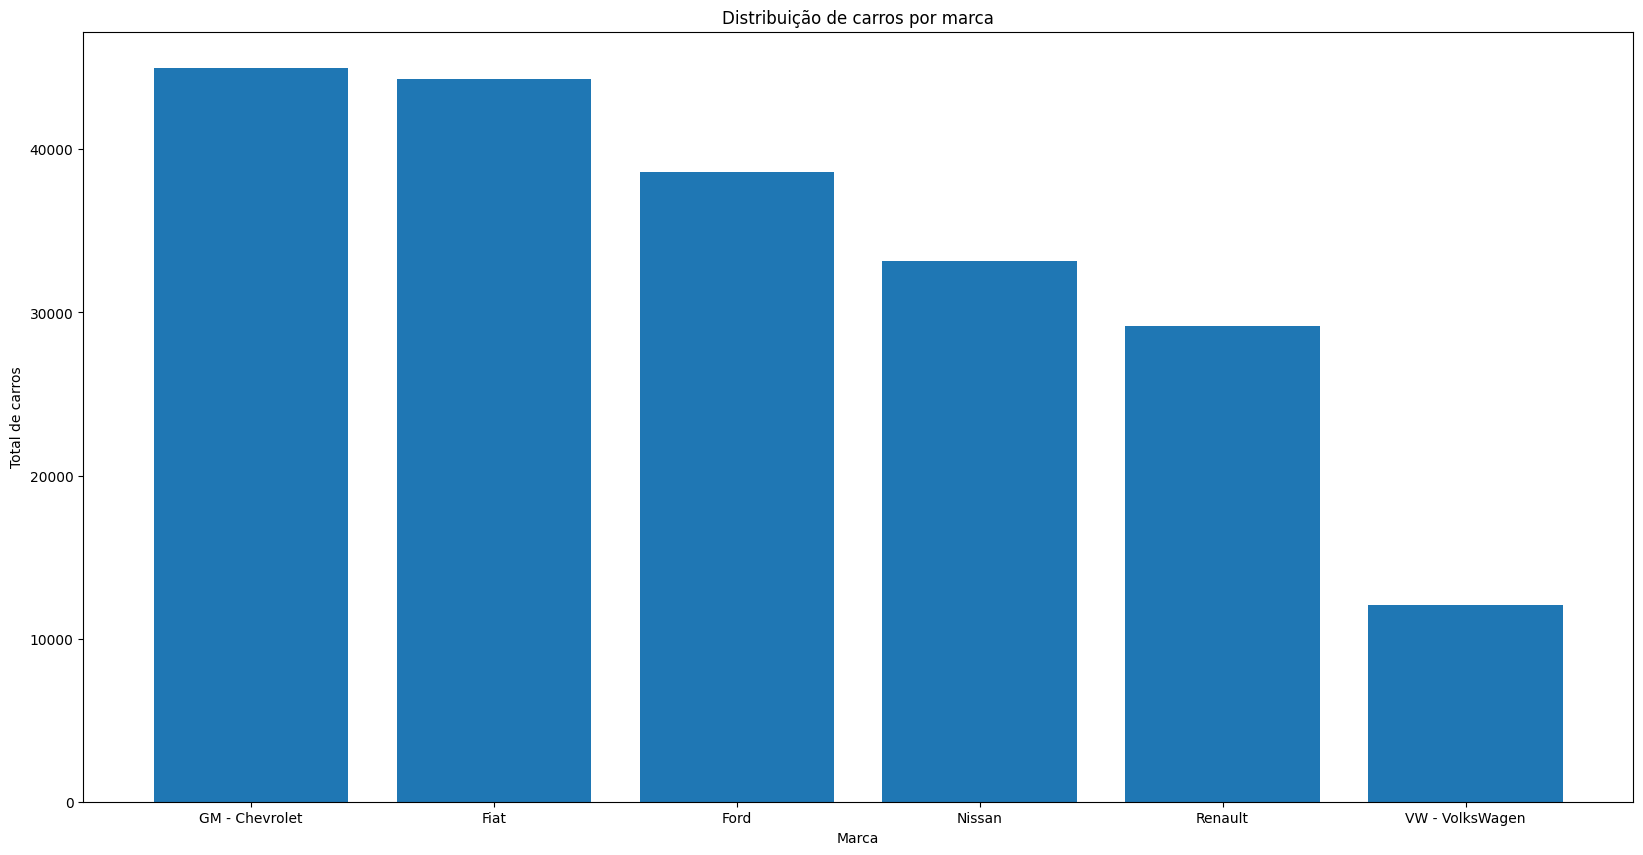
\includegraphics[width=1\linewidth]{apendices/fig/2_IAA002_1.png}
\caption{Distribuição de carros por marca}
\end{figure}

\begin{adjustwidth}{1em}{}
\textbf{b. Gere um gráfico da distribuição da quantidade de carros por tipo de engrenagem do carro}
\end{adjustwidth}
\begin{lstlisting}[language=Python, style=input]
dados['gear'].value_counts()
\end{lstlisting}
\begin{lstlisting}[language=, style=output]
manual       161883
automatic     40412
Name: gear, dtype: int64
\end{lstlisting}
\begin{lstlisting}[language=Python, style=input]
# Gráfico da distribuição por engrenagem (tipo de marcha)
plt.figure(figsize=(20,10)) 
plt.bar(dados['gear'].unique(), dados['gear'].value_counts()) 
plt.title('Distribuição de carros por engrenagem (marcha)') 
plt.ylabel('Total de carros') 
plt.xlabel('Tipo de engrenagem (marcha)') 
\end{lstlisting}
\begin{figure}[H]
\centering
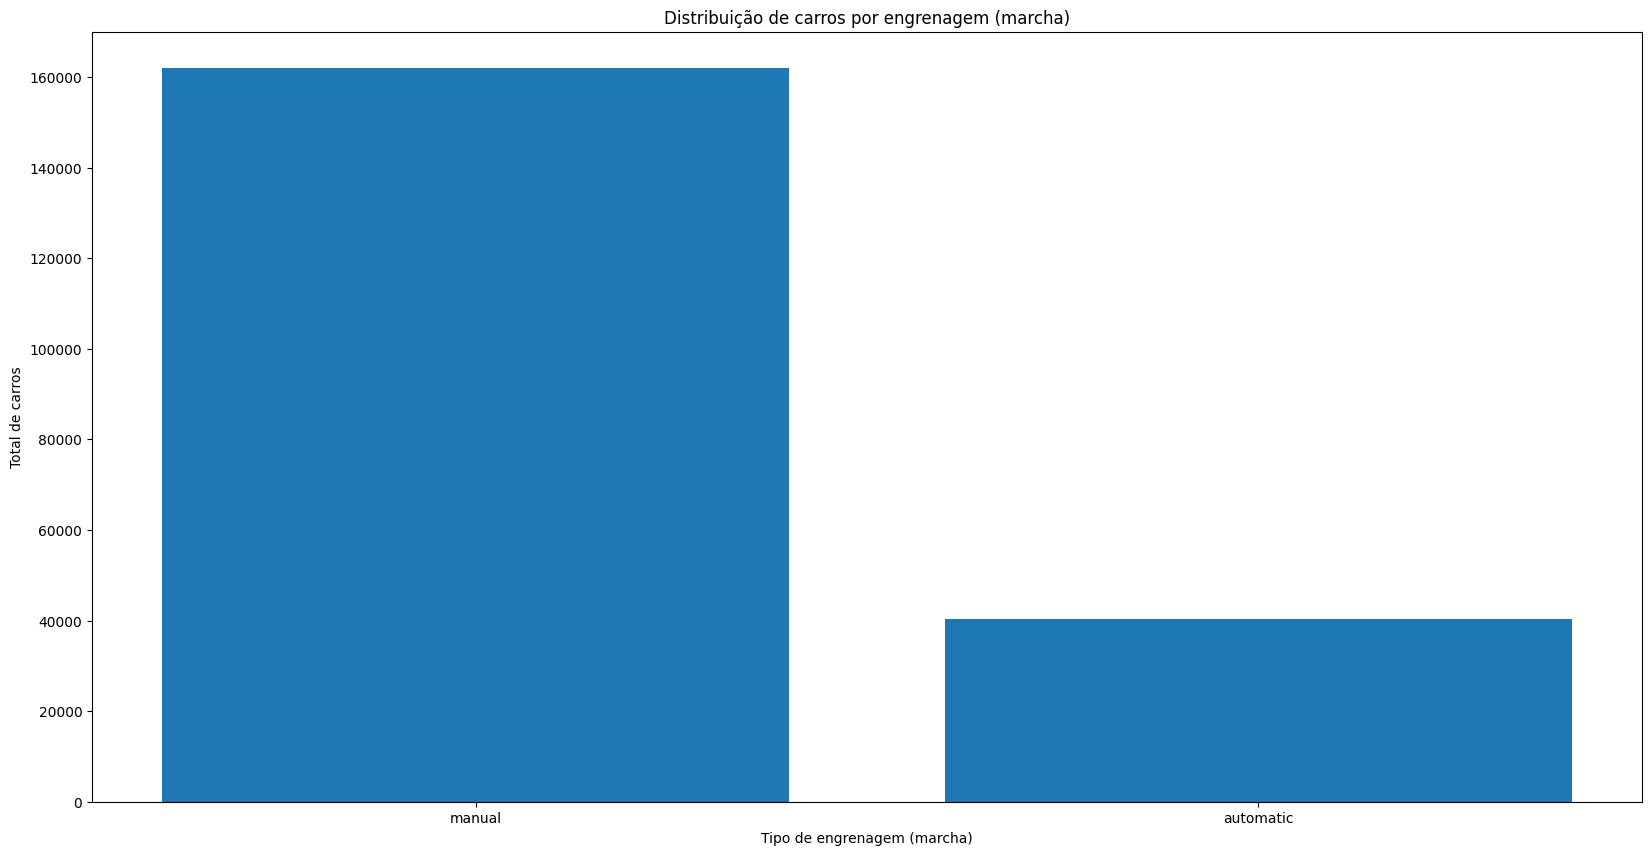
\includegraphics[width=1\linewidth]{apendices/fig/2_IAA002_2.png}
\caption{Distribuição de carros por engrenagem (marcha)}
\end{figure}

\begin{adjustwidth}{1em}{}
\textbf{c. Gere um gráfico da evolução da média de preço dos carros ao longo dos meses de 2022 (variável de tempo no eixo X)}
\end{adjustwidth}
\begin{lstlisting}[language=Python, style=input]
# limitando para somente os dados de 2022
dados_2022 = dados[dados['year_of_reference'] == 2022]
dados_2022.head()
\end{lstlisting}
\begin{table}[H]
\centering
\resizebox{\textwidth}{!}{
\begin{tabular}{lllllllllllll}
\hline
\textbf{ID} & \textbf{year\_ref} & \textbf{month} & \textbf{fipe\_code} & \textbf{auth} & \textbf{brand} & \textbf{model} & \textbf{fuel} & \textbf{gear} & \textbf{engine} & \textbf{year\_model} & \textbf{avg\_price} \\
\hline
96280 & 2022.0 & January & 004001-0 & gzw0hkct8cj4 & GM - Chevrolet & Corsa Wind 1.0 MPFI / EFI 2p & Gasoline & manual & 1 & 2002.0 & 12330.0 \\
96281 & 2022.0 & January & 004001-0 & gm2ws5yqjnfx & GM - Chevrolet & Corsa Wind 1.0 MPFI / EFI 2p & Gasoline & manual & 1 & 2001.0 & 11408.0 \\
96282 & 2022.0 & January & 004001-0 & gbvgy7432kp & GM - Chevrolet & Corsa Wind 1.0 MPFI / EFI 2p & Gasoline & manual & 1 & 2000.0 & 10620.0 \\
96283 & 2022.0 & January & 004001-0 & gvx412fg8v0 & GM - Chevrolet & Corsa Wind 1.0 MPFI / EFI 2p & Alcohol & manual & 1 & 2000.0 & 11992.0 \\
96284 & 2022.0 & January & 004003-7 & jtskpmg524fx & GM - Chevrolet & Corsa Pick-Up GL/ Champ 1.6 MPFI / EFI & Gasoline & manual & 1,6 & 2001.0 & 17182.0 \\
\hline
\end{tabular}
}
%caption{Sample vehicle listings from 2022}
\label{tab:vehicle_listings}
\end{table}
\begin{lstlisting}[language=Python, style=input]
# verificando os completude dos meses
dados_2022['month_of_reference'].drop_duplicates()
\end{lstlisting}
\begin{lstlisting}[language=, style=output]
96280       January
104390     February
112513        March
120665        April
128756          May
136850         June
144992         July
153143       August
161294    September
169483      October
177685     November
185880     December
Name: month_of_reference, dtype: object
\end{lstlisting}
\begin{lstlisting}[language=Python, style=input]
# Calculando a média de preços por mês
media_precos_mes = dados_2022.groupby(['year_of_reference','month_of_reference'])['avg_price_brl'].mean().round(0) 
df_media_precos_mes = media_precos_mes.reset_index(name='Médio de Preço')

# Reordenando o dataframe para melhor exibição no gráfico
df_media_precos_mes.insert(0, "index", [3,7,11,1,0,6,5,2,4,10,9,8], True)
df_media_precos_mes = df_media_precos_mes.sort_values(by=['index'])
df_media_precos_mes.head(12)
\end{lstlisting}
\begin{table}[H]
\centering
\begin{tabular}{rrrrl}
\hline
\textbf{Index} & \textbf{Order} & \textbf{Year} & \textbf{Month} & \textbf{Average Price (BRL)} \\
\hline
4 & 0 & 2022.0 & January & 54840.0 \\
3 & 1 & 2022.0 & February & 55825.0 \\
7 & 2 & 2022.0 & March & 56849.0 \\
0 & 3 & 2022.0 & April & 57150.0 \\
8 & 4 & 2022.0 & May & 57800.0 \\
6 & 5 & 2022.0 & June & 58066.0 \\
5 & 6 & 2022.0 & July & 57894.0 \\
1 & 7 & 2022.0 & August & 57924.0 \\
11 & 8 & 2022.0 & September & 58199.0 \\
10 & 9 & 2022.0 & October & 58227.0 \\
9 & 10 & 2022.0 & November & 58216.0 \\
2 & 11 & 2022.0 & December & 57997.0 \\
\hline
\end{tabular}
%\caption{Average monthly vehicle prices in 2022}
\label{tab:avg_price_2022}
\end{table}
\begin{lstlisting}[language=Python, style=input]
# Visualizando a média salarial por ano
plt.figure(figsize=(20,10)) 
sns.barplot(data=df_media_precos_mes, x='month_of_reference', y='Médio de Preço', hue='year_of_reference')
plt.ylim(50000, 60000) # limitação do eixo Y para melhor observação da variação de valores
plt.xticks(rotation=45);
\end{lstlisting}
\begin{figure}[H]
\centering
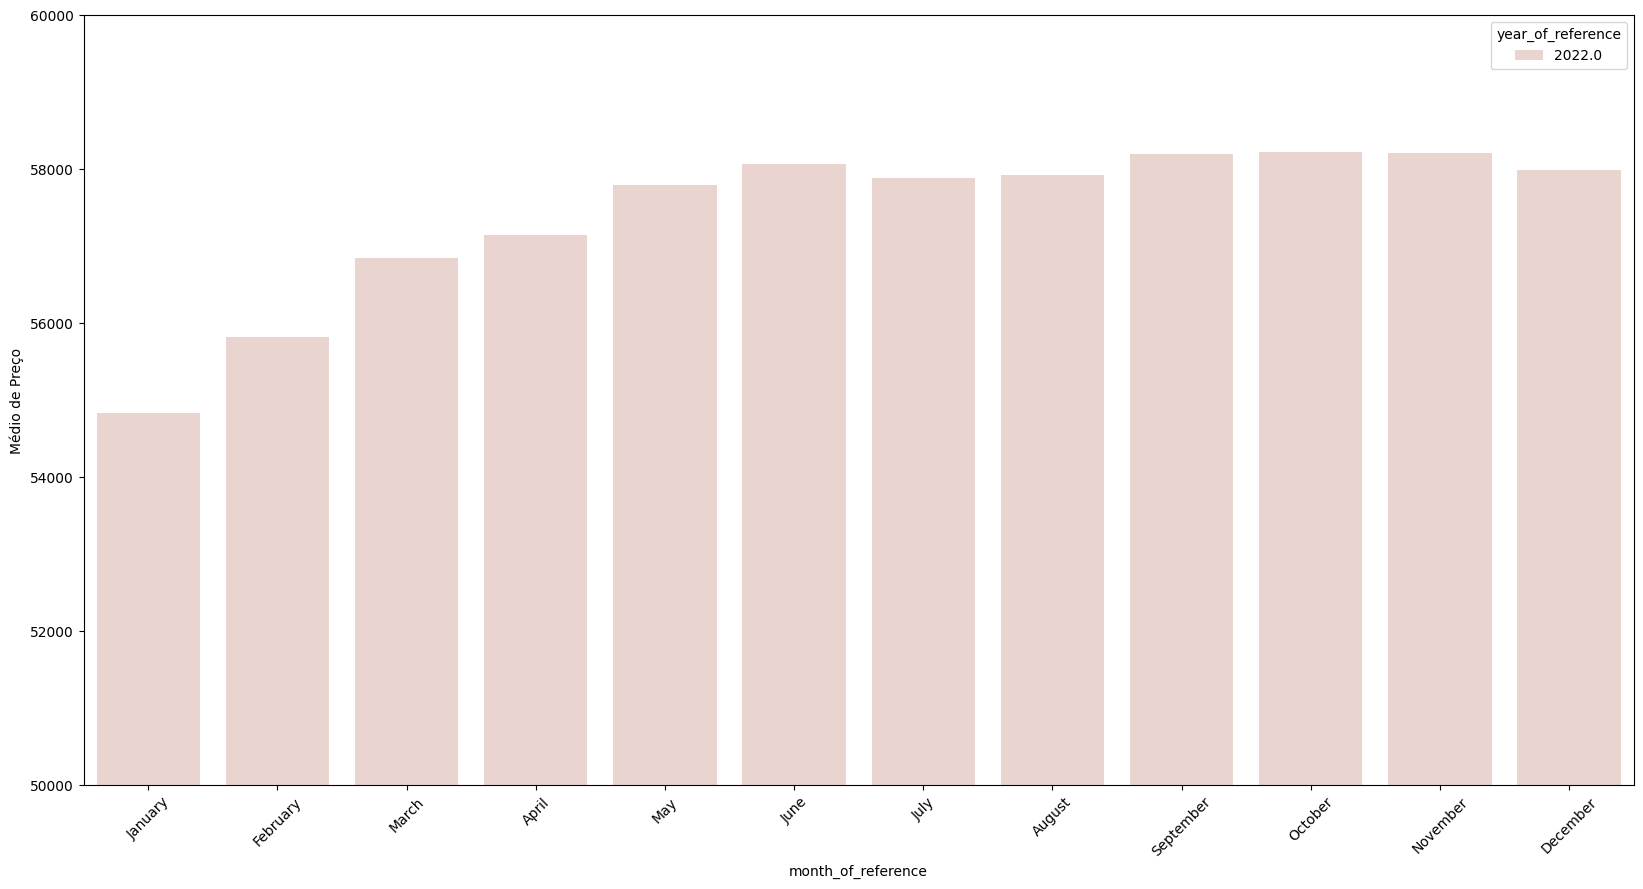
\includegraphics[width=1\linewidth]{apendices/fig/2_IAA002_3.png}
\caption{Evolução da média de preço dos carros ao longo dos meses de 2022}
\end{figure}



\begin{adjustwidth}{1em}{}
\textbf{d. Gere um gráfico da distribuição da média de preço dos carros por marca e tipo de engrenagem}
\end{adjustwidth}
\begin{lstlisting}[language=Python, style=input]
print(dados["gear"].unique()) # verificar os valores da coluna gear
\end{lstlisting}
\begin{lstlisting}[language=, style=output]
['manual' 'automatic']
\end{lstlisting}
\begin{lstlisting}[language=Python, style=input]
plt.figure(figsize=(20,10))
sns.barplot(x='brand', y='avg_price_brl', hue='gear', data=dados, hue_order=['manual', 'automatic'])
\end{lstlisting}
\begin{figure}[H]
\centering
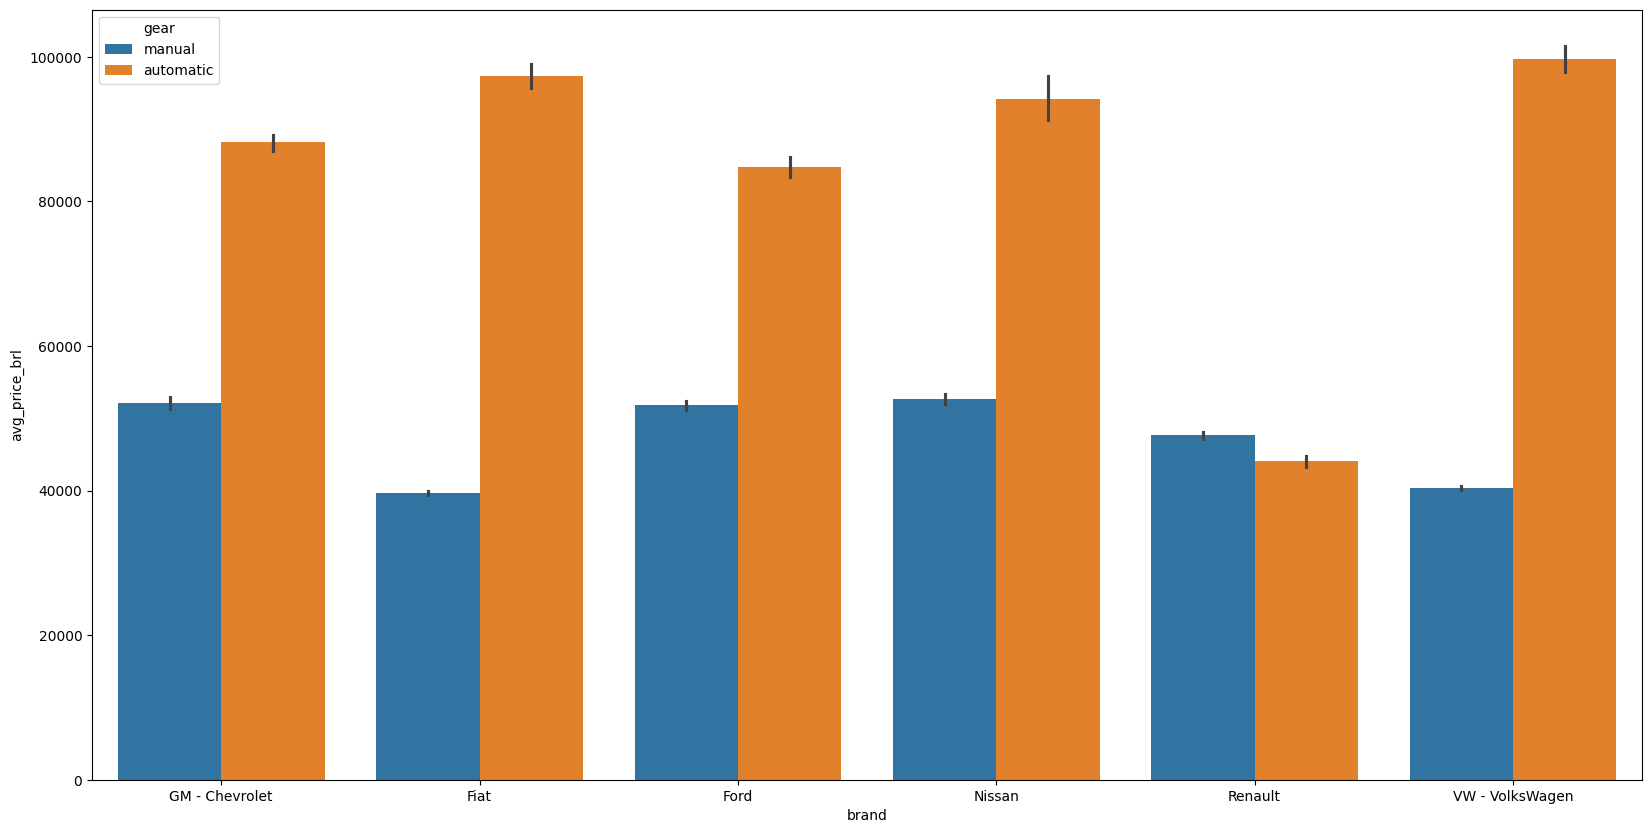
\includegraphics[width=1\linewidth]{apendices/fig/2_IAA002_4.png}
\caption{Distribuição da média de preço dos carros por marca e tipo de engrenagem}
\end{figure}

\begin{adjustwidth}{1em}{}
\textbf{e. Dê uma breve explicação (máximo de quatro linhas) sobre os resultados gerados no item d}
\end{adjustwidth}

O preço médio de carros com engrenagem (marcha) automática é superior aos com engrenagem manual em 5 das 6 marcas. Somente a Renault tem preços médios com ligeira superioridade nos carros com engrenagem manual. Nas marcas Fiat e Volkswagem os carro com engrenagem automática tem preço médio maiores do que o dobro dos carros com engrenagem manual.

\begin{adjustwidth}{1em}{}
\textbf{f. Gere um gráfico da distribuição da média de preço dos carros por marca e tipo de combustível}
\end{adjustwidth}
\begin{lstlisting}[language=Python, style=input]
print(dados["fuel"].unique()) # verificar os valores da coluna fuel
\end{lstlisting}
\begin{lstlisting}[language=, style=output]
['Gasoline' 'Alcohol' 'Diesel']
\end{lstlisting}
\begin{lstlisting}[language=Python, style=input]
plt.figure(figsize=(20,10))
sns.barplot(x='brand', y='avg_price_brl', hue='fuel', data=dados, hue_order=['Diesel', 'Gasoline', 'Alcohol'])
\end{lstlisting}
\begin{figure}[H]
\centering
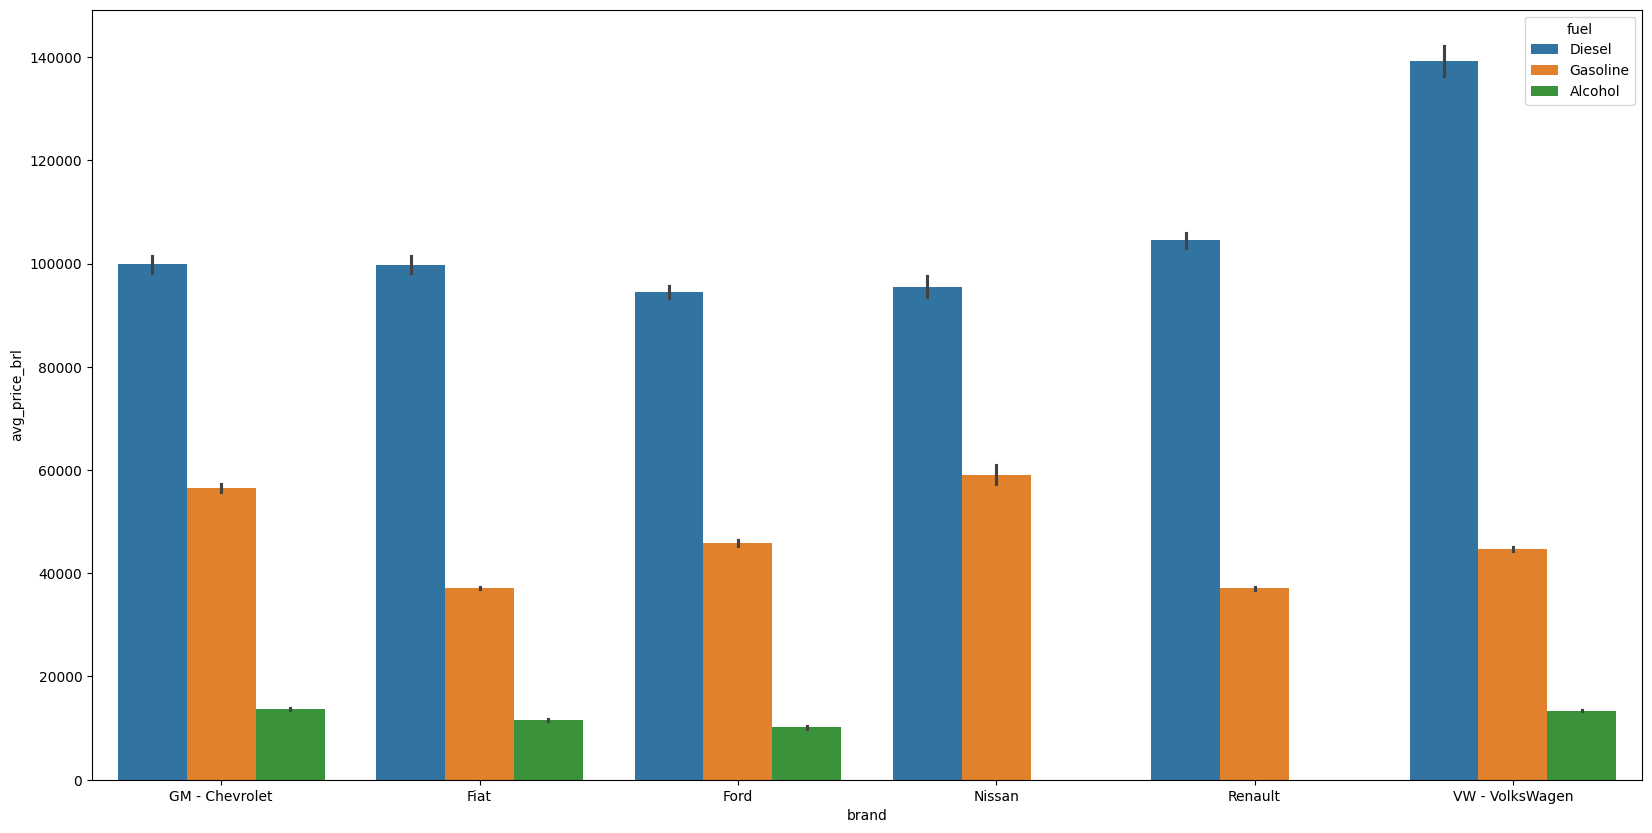
\includegraphics[width=1\linewidth]{apendices/fig/2_IAA002_5.png}
\caption{Distribuição da média de preço dos carros por marca e tipo de combustível}
\end{figure}

\begin{adjustwidth}{1em}{}
\textbf{g. Dê uma breve explicação (máximo de quatro linhas) sobre os resultados gerados no item f}
\end{adjustwidth}

Carros com o combustível Diesel tem os maiores preços médios em todas as marcas. O que faz sentido haja visto que motores a Diesel são comumente encontrados em carros maiores e de maiores valores. Veículos a Gasolina são os segundos com maiores preços médios em todas as marcas. Vale salientar que, nesta base, os veículos Flex (que podem consumir álcool e gasolina) estão categorizados como Gasolina.  Veículos a Álcool tem os menores preços médios nas marcas GM, Fiat, Ford e VM. As marcas Nissan e Renault não apresentaram veículos com combustível álcool.


\subsection*{\textbf{3 Aplicação de modelos de machine learning para prever o preço médio dos carros}}

\begin{adjustwidth}{1em}{}
\textbf{a. Escolha as variáveis \textbf{numéricas} (modelos de Regressão) para serem as variáveis independentes do modelo. A
variável target é \textbf{avg\_price. Observação:} caso julgue necessário, faça a transformação de variáveis
categóricas em variáveis numéricas para inputar no modelo. Indique \textbf{quais variáveis} foram transformadas e
\textbf{como} foram transformadas}
\end{adjustwidth}

\begin{lstlisting}[language=Python, style=input]
sns.boxplot(dados['avg_price_brl']).set_title("Distribuição dos preços dos carros") 
\end{lstlisting}
\begin{figure}[H]
\centering
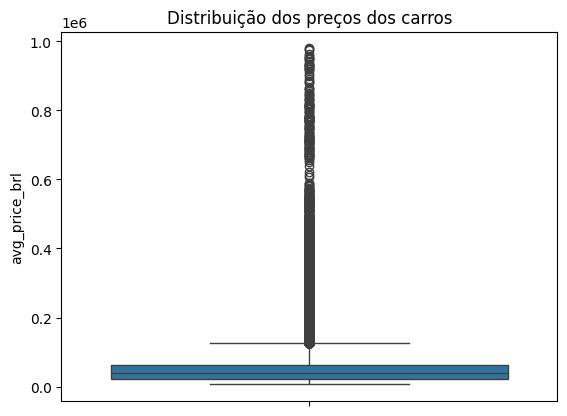
\includegraphics[width=.8\linewidth]{apendices/fig/2_IAA002_6.png}
\caption{Distribuição dos preços dos carros}
\end{figure}
\begin{lstlisting}[language=Python, style=input]
# Transformação da coluna modelo (model) de categórica para numérica
dados['model'] = LabelEncoder().fit_transform(dados['model']) 
dados.head()
\end{lstlisting}
\begin{table}[H]
\centering
\resizebox{\textwidth}{!}{
\begin{tabular}{rrrrllllllll}
\hline
\textbf{ID} & \textbf{Year} & \textbf{Month} & \textbf{FIPE Code} & \textbf{Auth} & \textbf{Brand} & \textbf{Model Code} & \textbf{Fuel} & \textbf{Gear} & \textbf{Engine} & \textbf{Year Model} & \textbf{Avg. Price (BRL)} \\
\hline
0 & 2021.0 & January & 004001-0 & cfzlctzfwrcp & GM - Chevrolet & 297 & Gasoline & manual & 1 & 2002.0 & 9162.0 \\
1 & 2021.0 & January & 004001-0 & cdqwxwpw3y2p & GM - Chevrolet & 297 & Gasoline & manual & 1 & 2001.0 & 8832.0 \\
2 & 2021.0 & January & 004001-0 & cb1t3xwwj1xp & GM - Chevrolet & 297 & Gasoline & manual & 1 & 2000.0 & 8388.0 \\
3 & 2021.0 & January & 004001-0 & cb9gct6j65r0 & GM - Chevrolet & 297 & Alcohol & manual & 1 & 2000.0 & 8453.0 \\
4 & 2021.0 & January & 004003-7 & g15wg0gbz1fx & GM - Chevrolet & 260 & Gasoline & manual & 1,6 & 2001.0 & 12525.0 \\
\hline
\end{tabular}
}
%\caption{Sample vehicle price records for January 2021}
\label{tab:vehicle_prices_jan2021}
\end{table}
\begin{lstlisting}[language=Python, style=input]
# Transformação da coluna engrenagem (gear) de categórica para numérica
dados['gear'] = LabelEncoder().fit_transform(dados['gear']) 
dados.head()
\end{lstlisting}
\begin{table}[H]
\centering
\resizebox{\textwidth}{!}{
\begin{tabular}{rrrrllllllll}
\hline
\textbf{ID} & \textbf{Year} & \textbf{Month} & \textbf{FIPE Code} & \textbf{Auth} & \textbf{Brand} & \textbf{Model} & \textbf{Fuel} & \textbf{Gear} & \textbf{Engine} & \textbf{Year Model} & \textbf{Avg. Price (BRL)} \\
\hline
0 & 2021.0 & January & 004001-0 & cfzlctzfwrcp & GM - Chevrolet & 297 & Gasoline & 1 & 1 & 2002.0 & 9162.0 \\
1 & 2021.0 & January & 004001-0 & cdqwxwpw3y2p & GM - Chevrolet & 297 & Gasoline & 1 & 1 & 2001.0 & 8832.0 \\
2 & 2021.0 & January & 004001-0 & cb1t3xwwj1xp & GM - Chevrolet & 297 & Gasoline & 1 & 1 & 2000.0 & 8388.0 \\
3 & 2021.0 & January & 004001-0 & cb9gct6j65r0 & GM - Chevrolet & 297 & Alcohol  & 1 & 1 & 2000.0 & 8453.0 \\
4 & 2021.0 & January & 004003-7 & g15wg0gbz1fx & GM - Chevrolet & 260 & Gasoline & 1 & 1,6 & 2001.0 & 12525.0 \\
\hline
\end{tabular}
}
%\caption{Vehicle pricing data from January 2021}
\label{tab:jan2021_vehicle_prices}
\end{table}
\begin{lstlisting}[language=Python, style=input]
# Transformação da coluna combustível (fuel) de categórica para numérica
dados['fuel'] = LabelEncoder().fit_transform(dados['fuel']) 
dados.head()
\end{lstlisting}
\begin{table}[H]
\centering
\resizebox{\textwidth}{!}{
\begin{tabular}{rrrrllllllll}
\hline
\textbf{ID} & \textbf{Year} & \textbf{Month} & \textbf{FIPE Code} & \textbf{Auth} & \textbf{Brand} & \textbf{Model} & \textbf{Fuel} & \textbf{Gear} & \textbf{Engine} & \textbf{Year Model} & \textbf{Avg. Price (BRL)} \\
\hline
0 & 2021.0 & January & 004001-0 & cfzlctzfwrcp & GM - Chevrolet & 297 & 2 & 1 & 1 & 2002.0 & 9162.0 \\
1 & 2021.0 & January & 004001-0 & cdqwxwpw3y2p & GM - Chevrolet & 297 & 2 & 1 & 1 & 2001.0 & 8832.0 \\
2 & 2021.0 & January & 004001-0 & cb1t3xwwj1xp & GM - Chevrolet & 297 & 2 & 1 & 1 & 2000.0 & 8388.0 \\
3 & 2021.0 & January & 004001-0 & cb9gct6j65r0 & GM - Chevrolet & 297 & 0 & 1 & 1 & 2000.0 & 8453.0 \\
4 & 2021.0 & January & 004003-7 & g15wg0gbz1fx & GM - Chevrolet & 260 & 2 & 1 & 1,6 & 2001.0 & 12525.0 \\
\hline
\end{tabular}
}
%\caption{Vehicle data with numeric codes for fuel and gear types}
\label{tab:vehicle_data_encoded}
\end{table}
\begin{lstlisting}[language=Python, style=input]
dados.columns
\end{lstlisting}
\begin{lstlisting}[language=, style=output]
Index(['year_of_reference', 'month_of_reference', 'fipe_code',
       'authentication', 'brand', 'model', 'fuel', 'gear', 'engine_size',
       'year_model', 'avg_price_brl'],
      dtype='object')
\end{lstlisting}
\begin{lstlisting}[language=Python, style=input]
# Variável dados_num contém apenas variáveis numéricas de interesse (exclui o restante)
dados_num = dados.drop(['year_of_reference', 'month_of_reference', 'fipe_code', 'authentication', 'brand', 'engine_size'],axis = 1)
dados_num.head()
\end{lstlisting}
\begin{table}[H]
%\begin{table}[h!]
\centering
\begin{tabular}{rrrrr}
\hline
\textbf{Model Code} & \textbf{Fuel Code} & \textbf{Gear Code} & \textbf{Year Model} & \textbf{Avg. Price (BRL)} \\
\hline
297 & 2 & 1 & 2002.0 & 9162.0 \\
297 & 2 & 1 & 2001.0 & 8832.0 \\
297 & 2 & 1 & 2000.0 & 8388.0 \\
297 & 0 & 1 & 2000.0 & 8453.0 \\
260 & 2 & 1 & 2001.0 & 12525.0 \\
\hline
\end{tabular}
%\caption{Simplified vehicle data with numeric fuel and gear codes}
\label{tab:simplified_vehicle_data}
\end{table}
\begin{lstlisting}[language=Python, style=input]
dados_num.dtypes
\end{lstlisting}
\begin{lstlisting}[language=, style=output]
model              int32
fuel               int32
gear               int32
year_model       float64
avg_price_brl    float64
dtype: object
\end{lstlisting}
\begin{lstlisting}[language=Python, style=input]
sns.heatmap(dados_num.corr("spearman"), annot = True)
plt.title("Mapa de Correlação das Variáveis Numéricas\n", fontsize = 15)
plt.show()
\end{lstlisting}
\begin{figure}[H]
\centering
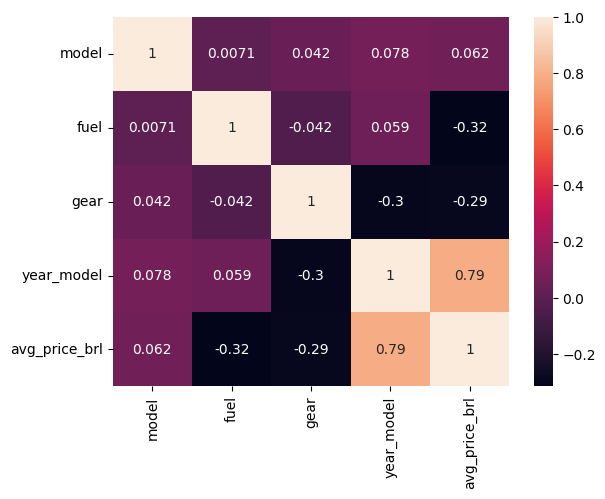
\includegraphics[width=.8\linewidth]{apendices/fig/2_IAA002_7.png}
\caption{Mapa de Correlação das Variáveis Numéricas}
\end{figure}
\begin{lstlisting}[language=Python, style=input]
# Variável X contém apenas variáveis numéricas de interesse para a análise, excluindo a variável target 
X = dados_num.drop(['avg_price_brl'],axis = 1)
X.head()
\end{lstlisting}
\begin{table}[H]
\centering
\begin{tabular}{rrrr}
\hline
\textbf{Model Code} & \textbf{Fuel Code} & \textbf{Gear Code} & \textbf{Year Model} \\
\hline
297 & 2 & 1 & 2002.0 \\
297 & 2 & 1 & 2001.0 \\
297 & 2 & 1 & 2000.0 \\
297 & 0 & 1 & 2000.0 \\
260 & 2 & 1 & 2001.0 \\
\hline
\end{tabular}
%\caption{Basic vehicle specifications by model, fuel, gear, and year}
\label{tab:vehicle_specs}
\end{table}
\begin{lstlisting}[language=Python, style=input]
Y = dados_num['avg_price_brl']
Y.head()
\end{lstlisting}
\begin{lstlisting}[language=, style=output]
0     9162.0
1     8832.0
2     8388.0
3     8453.0
4    12525.0
Name: avg_price_brl, dtype: float64
\end{lstlisting}





\begin{adjustwidth}{1em}{}
\textbf{b. Crie partições contendo 75\% dos dados para treino e 25\% para teste}
\end{adjustwidth}
\begin{lstlisting}[language=Python, style=input]
# Divisão: 30% dos dados são de teste e 70% de treinamento
X_train, X_test, Y_train, Y_test = train_test_split(X, Y, test_size = 0.25, random_state = 42)

# Observando os dados de treinamento
print(X_train.shape)
X_train.head()
\end{lstlisting}
\begin{table}[H]
\centering
\begin{tabular}{rrrr}
\hline
\textbf{Model Code} & \textbf{Fuel Code} & \textbf{Gear Code} & \textbf{Year Model} \\
\hline
364  & 1 & 1 & 2020.0 \\
1099 & 2 & 1 & 2011.0 \\
549  & 2 & 1 & 2008.0 \\
385  & 1 & 1 & 2013.0 \\
970  & 2 & 1 & 2018.0 \\
\hline
\end{tabular}
%\caption{Vehicle model, fuel type, gear type, and year}
\label{tab:model_fuel_gear_year}
\end{table}
\begin{lstlisting}[language=Python, style=input]
# Observando os dados de teste
print(X_test.shape)
X_test.head()
\end{lstlisting}
\begin{table}[H]
\centering
\begin{tabular}{rrrr}
\hline
\textbf{Model Code} & \textbf{Fuel Code} & \textbf{Gear Code} & \textbf{Year Model} \\
\hline
1235 & 2 & 1 & 2015.0 \\
224  & 2 & 1 & 2005.0 \\
1984 & 2 & 1 & 2003.0 \\
1114 & 2 & 1 & 2008.0 \\
310  & 2 & 0 & 2019.0 \\
\hline
\end{tabular}
%\caption{Vehicle model info with fuel, gear type, and year}
\label{tab:model_info_fuel_gear}
\end{table}
\begin{lstlisting}[language=Python, style=input]
# Observando a variável target
Y_test.head()
\end{lstlisting}
\begin{lstlisting}[language=, style=output]
180633    42595.0
13130     10989.0
163315     9087.0
121464    26965.0
14044     57102.0
Name: avg_price_brl, dtype: float64
\end{lstlisting}



\begin{adjustwidth}{1em}{}
\textbf{c. Treine modelos RandomForest (biblioteca RandomForestRegressor) e XGBoost (biblioteca XGBRegressor) para predição
dos preços dos carros. \textbf{Observação}: caso julgue necessário, mude os parâmetros dos modelos e rode novos
modelos. Indique quais parâmetros foram inputados e indique o treinamento de cada modelo}
\end{adjustwidth}
\begin{lstlisting}[language=Python, style=input]
#RandomForest
model_rf = RandomForestRegressor()
model_rf.fit(X_train, Y_train)
\end{lstlisting}

\begin{lstlisting}[language=Python, style=input]
#RandomForest com parâmetros
n_estimators = [5,20,50,100] # number of trees in the random forest
max_features = ['auto', 'sqrt'] # number of features in consideration at every split
max_depth = [int(x) for x in np.linspace(10, 120, num = 12)] # maximum number of levels allowed in each decision tree
min_samples_split = [2, 6, 10] # minimum sample number to split a node
min_samples_leaf = [1, 3, 4] # minimum sample number that can be stored in a leaf node
bootstrap = [True, False] # method used to sample data points

random_grid = {'n_estimators': n_estimators, 'max_features': max_features, 'max_depth': max_depth, 'min_samples_split': min_samples_split, 
               'min_samples_leaf': min_samples_leaf, 'bootstrap': bootstrap}

rf = RandomForestRegressor()
rf_random = RandomizedSearchCV(estimator = rf,param_distributions = random_grid,
               n_iter = 100, cv = 5, verbose=2, random_state=35, n_jobs = -1)

rf_random.fit(X_train, Y_train)

# Utilizando os melhores parâmetros encontrados
model_rf_parametros = RandomForestRegressor(max_depth=70, min_samples_leaf=1, min_samples_split=2, n_estimators=20, random_state=80)

model_rf_parametros.fit(X_train, Y_train)
\end{lstlisting}

\begin{lstlisting}[language=Python, style=input]
#XGBoost
model_xgboost = XGBRegressor()
model_xgboost.fit(X_train, Y_train)
\end{lstlisting}


\begin{adjustwidth}{1em}{}
\textbf{d. Grave os valores preditos em variáveis criadas}
\end{adjustwidth}
\begin{lstlisting}[language=Python, style=input]
#RandomForest
valores_preditos_rf = model_rf.predict(X_test)
valores_preditos_rf 
\end{lstlisting}
\begin{lstlisting}[language=, style=output]
array([ 40202.75425599,  13245.75443638,   8284.98551924, ...,
       100752.20098065,   9079.96883553,  26846.22919497])
\end{lstlisting}

\begin{lstlisting}[language=Python, style=input]
#RandomForest com parâmetros
valores_preditos_rf_parametros = model_rf_parametros.predict(X_test)
valores_preditos_rf_parametros
\end{lstlisting}
\begin{lstlisting}[language=, style=output]
array([ 40228.52250094,  13256.95619505,   8173.31940763, ...,
       101226.60508665,   9092.06259221,  27167.56218788])
\end{lstlisting}

\begin{lstlisting}[language=Python, style=input]
#XGBoost
valores_preditos_xgboost = model_xgboost.predict(X_test)
valores_preditos_xgboost
\end{lstlisting}
\begin{lstlisting}[language=, style=output]
array([40623.945, 13863.4  ,  8653.945, ..., 99269.16 , 10503.629,
       25664.008], dtype=float32)
\end{lstlisting}

\begin{adjustwidth}{1em}{}
\textbf{e. Realize a análise de importância das variáveis para estimar a variável target, \textbf{para cada modelo treinado}}
\end{adjustwidth}
\begin{lstlisting}[language=Python, style=input]
#RandomForest
model_rf.feature_importances_
feature_importances_rf = pd.DataFrame(model_rf.feature_importances_, index = X_train.columns, columns=['importance']).sort_values('importance', ascending = False)
feature_importances_rf 
\end{lstlisting}
\begin{table}[H]
\centering
\begin{tabular}{lr}
\hline
\textbf{Feature} & \textbf{Importance} \\
\hline
model      & 0.439964 \\
year\_model & 0.358480 \\
fuel       & 0.179241 \\
gear       & 0.022315 \\
\hline
\end{tabular}
%\caption{Feature importance values}
\label{tab:feature_importance}
\end{table}


\begin{lstlisting}[language=Python, style=input]
#RandomForest com parâmetros
model_rf_parametros.feature_importances_
feature_importances_rf_param = pd.DataFrame(model_rf_parametros.feature_importances_, index = X_train.columns, columns=['importance']).sort_values('importance', ascending = False)
feature_importances_rf_param
\end{lstlisting}
\begin{table}[H]
\centering
\begin{tabular}{lr}
\hline
\textbf{Feature} & \textbf{Importance} \\
\hline
model       & 0.442857 \\
year\_model & 0.356757 \\
fuel        & 0.178231 \\
gear        & 0.022155 \\
\hline
\end{tabular}
%\caption{Updated feature importance values}
\label{tab:updated_feature_importance}
\end{table}


\begin{lstlisting}[language=Python, style=input]
#XGBoost
model_xgboost.feature_importances_
feature_importances_x = pd.DataFrame(model_xgboost.feature_importances_, index = X_train.columns, columns=['importance']).sort_values('importance', ascending = False)
feature_importances_x
\end{lstlisting}
\begin{table}[H]
\centering
\begin{tabular}{lr}
\hline
\textbf{Feature} & \textbf{Importance} \\
\hline
fuel        & 0.699523 \\
year\_model & 0.160642 \\
model       & 0.088919 \\
gear        & 0.050917 \\
\hline
\end{tabular}
%\caption{Feature importance values (latest version)}
\label{tab:feature_importance_latest}
\end{table}



\begin{adjustwidth}{1em}{}
\textbf{f. Dê uma breve explicação (máximo de quatro linhas) sobre os resultados encontrados na análise de importância de
variáveis}
\end{adjustwidth}

Tanto no modelo Random Forest, quando no modelo Random Forest com parâmetros, as variáveis mais importantes foram modelo e ano do modelo (model e year\_model) com quse 80\% de importância. Somando a combustível (fuel) chegamos a 97\% de importância. Tornando quase irrelevante a variável engrenagem (gear). Para o modelo XGBoost temos como variável mais importante o combustível (fuel) com aproximadamente 70\% e seguido de ano do modelo com 16\%. Modelo e engrenagem (model e gear) aparecem com menos de 10\% cada.

\begin{adjustwidth}{1em}{}
\textbf{g. Escolha o melhor modelo com base nas métricas de avaliação MSE, MAE e R²}
\end{adjustwidth}
\begin{lstlisting}[language=Python, style=input]
#RandomForest
mse_rf = mean_squared_error(Y_test, valores_preditos_rf)
mae_rf = mean_absolute_error(Y_test, valores_preditos_rf)
r2_rf = r2_score(Y_test, valores_preditos_rf)
mse_rf
mae_rf
r2_rf
\end{lstlisting}
\begin{lstlisting}[language=, style=output]
54633997.34991135
4215.705784378993
0.97969945241549
\end{lstlisting}


\begin{lstlisting}[language=Python, style=input]
#RandomForest com parâmetros
mse_rf_param = mean_squared_error(Y_test, valores_preditos_rf_parametros)
mae_rf_param = mean_absolute_error(Y_test, valores_preditos_rf_parametros)
r2_rf_param = r2_score(Y_test, valores_preditos_rf_parametros)
mse_rf_param
mae_rf_param
r2_rf_param
\end{lstlisting}
\begin{lstlisting}[language=, style=output]
54716253.201698475
4216.618281471371
0.9796688883177797
\end{lstlisting}


\begin{lstlisting}[language=Python, style=input]
#XGBoost
mse_x = mean_squared_error(Y_test, valores_preditos_xgboost)
mae_x = mean_absolute_error(Y_test, valores_preditos_xgboost)
r2_x = r2_score(Y_test, valores_preditos_xgboost)
mse_x
mae_x
r2_x
\end{lstlisting}
\begin{lstlisting}[language=, style=output]
297039446.66991967
6429.30300193814
0.8896280024509496
\end{lstlisting}

\begin{adjustwidth}{1em}{}
\textbf{h. Dê uma breve explicação (máximo de quatro linhas) sobre qual modelo gerou o melhor resultado e a métrica de
avaliação utilizada}
\end{adjustwidth}

Levando em conta a acurácia resultante da métrica R2, temos os seguintes resultados:
\begin{itemize}
    \item Random Forest: 98\%
    \item Random Forest com parâmetros: 98\%
    \item XGBoost: 89\%
\end{itemize}
Desta forma, temos um empate entre Random Forest e Random Forest com parâmetros. Para fins de entendimento, trazemos a comparação dos resultados de MSE e MAE (quanto menores, melhores os resultados):

\begin{itemize}
    \item MSE
    \begin{itemize}
        \item Random Forest: 54.622.503
        \item Random Forest com parâmetros: 54.716.253
    \end{itemize}
    \item MAE
    \begin{itemize}
        \item Random Forest: 4215
        \item Random Forest com parâmetros: 4217
    \end{itemize}
\end{itemize}

Como podemos ver, há uma ligeira vantagem no uso do Random Forest, sem parâmetros. Assim sendo, concluímos que o melhor resultado preditivo foi obtido através do modelo Random Forest.